\part{Validation}
%\setcounter{chapter}{0}

~\vspace{1cm}
\begin{flushright}
{\it Winners compare their achievements with their goals, while losers compare their achievements with those of other people.}\\
Nido Qubein
\end{flushright}
\vspace{2cm}

\enti{} was tested on a realistic use-case scenario, in which all previously-listed properties were stressed. This scenario, defined in collaboration with partners of an AAL project, is presented this chapter~\ref{ch:aalValidation}.\\

%A second validation has been realized by bringing \enti{} in front of a bundle of end-users, namely elderly people. This study had two goals. The first goal was the improvement of the \gls{gui} widgets presented to end-users, in order to make them as intuitive as possible. The second was the verification that people are able to act on, and get information from the home, according to a pre-define scenario. These two points are detailed in chapter~\ref{ch:itiProject}.\\


\chapter{Validation in the context of an AAL project}
\label{ch:aalValidation}

As one of the IDA project's partners, we proposed \enti{} as a flexible integration tool, for the different types of equipment offered by industrialists. \enti{} has been considered and evaluated on a scenario, collaboratively defined with the partners of the project. It has been designed to underline the properties required for such a system.\\

The first section of this chapter introduces the project and its context and details the scenario used as a validation for \enti{}. Sections~\ref{subsec:interop} to \ref{subsec:opening} describe the evaluation of a set of properties: the environment setup, the procedures, and the results for an evaluated property. Section~\ref{sec:theatsToValidity} lists some threats to the validity of this study. The conclusion and perspectives of these experiments is presented in section~\ref{sec:concluAAL}.

\section{Context of the study: the IDA project}

The first phase of the \gls{ida}~\footnote{http://www.ida-autonomie.fr/} project took place from June 2008 to June 2010, in the City of Rennes and the greater Rennes area(France). This local \gls{aal} project was funded by the Regional Council of Brittany to investigate issues resulting from the ageing of the population, and its socio-economic impact. More precisely, the \gls{ida} project involved conducting an inquiry about the use of \gls{ict} to help elderly people in their everyday life at home. To this end, the project involved:\\
\begin{itemize}
\item[{\bf Association for care at home}] ASSAD du Pays de Rennes
\item[{\bf Industrialists}] Custos, Delta Dore, Urmet Captive, Spartime, i--Pocarte, Domtis, Ordimemo, Intervox Systems, Laudren, Solem
\item[{\bf Social housing authority}] Archipel Habitat
\item[{\bf Installers}] Marsollier Domotique, Lepage Electronique
\item[{\bf Project ownership assistance}] ARELIA
\item[{\bf Research institutes}] INRIA (National Institute of Research in Computer Science and Control), the University of Rennes 1, the University of Rennes 2, LOUSTIC (Information and Communication technology Observation Laboratory), IETR (Rennes Electronics and Telecommunications Institute), CRPCC (Psychology, Cognition and Communication Research Center)
\item[{\bf Public administrations}] Rennes Metropole, Conseil General d'Ille et Vilaine, Ville de Rennes, CCI Rennes, Critt Santé, MEITO
\item[{\bf Elderly people}] Anonymous individuals for tests, obviously
\end{itemize}
The conclusions of the project have been compiled in \cite{ASSAD:2010}.\\

The "ASSAD du Pays de Rennes" Association, leader of this project, employs 450 persons among which, nurses, home care assistants, technicians, etc. The association helps more than 3,000 persons, in 17 towns in the south and east of Rennes.\\

Although the IDA was not funded by the European \gls{aal} program the assisted (elderly) person was project-centred, and the six dimensions described in section~\ref{subsec:aalConcepts} appeared in the background all throughout the project. The ASSAD association took care of this point.\\
\enti{} had been presented as a system for the integration of the several devices evaluated in the project. Indeed, the objective of IDA was to measure how \gls{ict} could foster the autonomy of elderly people at home and support the activity of carers. In this context, we proposed \enti{} as an integration platform, able to deal with various devices and services, and promote the deployment of solutions adapted to each person's needs.\\

Interested in the proposition, collaborative work had been engaged within the IDA project. With the help of the ASSAD, Delta Dore, Custos, Arelia, and the LOUSTIC, among the most active, a scenario was defined to put \enti{} in context.\\
This case study was designed to be as close as possible to real life conditions. The story was introduced by the ASSAD association. Products were proposed by Delta Dore. The evolutions were gathered from past experiences of the ASSAD, Custos and the LOUSTIC. This scenario was set up to evaluate \enti{} on a realistic case, with the same devices as those actually deployed. It stresses several issues to measure how \enti{} would cope with them.\\
The following part of this section presents the story and the evaluation context of \enti{}. The way \enti{} addressed the problems is described for each issue in a separate section.


\section{Use case and issues to address}
\label{sec:usecase}

The scenario used for the evaluation of \enti{} is presented in this section. It involves an elderly person called Mrs P., several members of her family, and different devices selected in collaboration with other partners in order for the evaluation to be realized with real products and in the closest conditions to reality.\\

The scenario is presented here with names of persons and real products for the sake of clarity.\\

The scenario is about Mrs P. She is seventy-eight. She has two children and five grandchildren. Mrs P. begins to experience some difficulties in walking and moving. To improve her safety, her daughter proposed that she moves to an equipped flat.\\
Among other equipment, the flat is basically equipped with an alert system, which triggers a voice call to a care center when a button is pressed on a remote control. But Mrs P. is not comfortable with this equipment and would prefer a more generic remote control. She also would like the alert to be sent to her daughter, instead of to the care center.\\

\begin{figure}[h!]
\centering
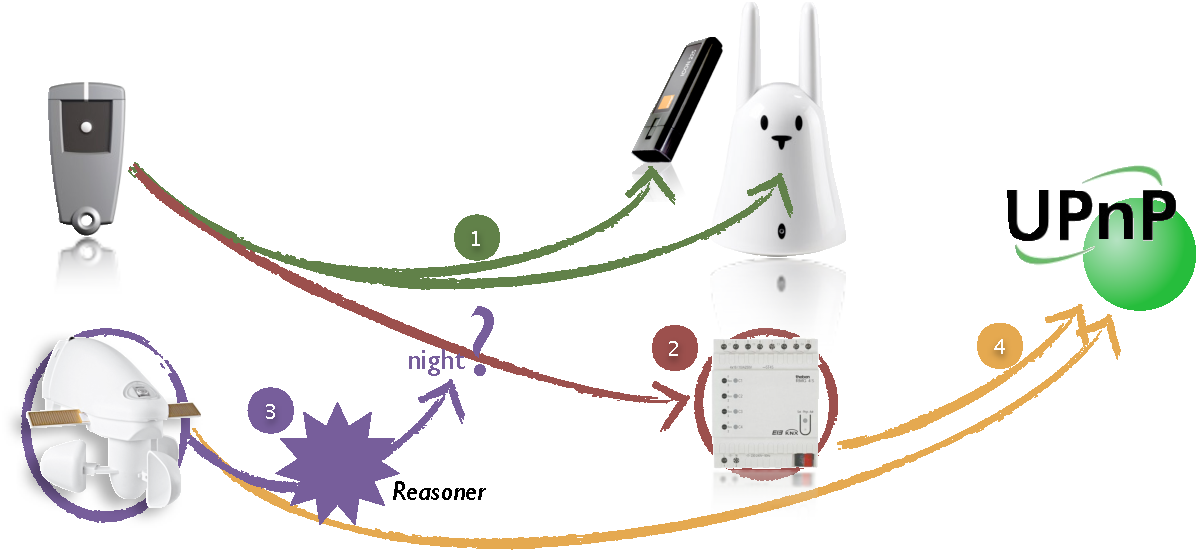
\includegraphics[width=.7\textwidth]{part4/pics/ConcreteApplication}
\caption{Solution elements for Mrs P.}
\label{fig:concreteApplication}
\end{figure}

The remote control, on the top left corner of figure~\ref{fig:concreteApplication}, is a one-button command from Delta Dore (a French manufacturer of home automation devices). This remote control has been designed to be universal for any receiver product from the Delta Dore catalog. A 3G-communication stick (Icon 225) is used to send alerts to Mrs P.'s daughter. Then a Nabaztag rabbit helpfully provides feedback to Mrs P. when she asks for help from her daughter.\\
The connection of these three items raises {\bf interoperability} problems (symbolized by the bullet number one), which are detailed and answered in section~\ref{subsec:interop}.\\

After some months of use, Mrs P. asks for the system to automatically switch on the lights, when an alert is sent. Luckily, the flat is already equipped with devices that enable the control of lights. The light control is made available by a \textit{RMG4S} device from Theben (on the bottom right of figure~\ref{fig:concreteApplication}, working on a KNX network. Section~\ref{subsec:evolution} presents how \enti{} enabled this {\bf evolution}.\\

Following this evolution, the behavior of the lights was sub-optimal, because the lights were switched on whatever the period of the day. To eliminate this issue, an {\bf adaptation} mechanism(bullet 3), described in section~\ref{subsec:adaptation}, was deployed. The sensing of daylight was realized by a KNX weather station outside the house. This weather station is visible on the bottom left corner of figure~\ref{fig:concreteApplication}.\\

One day, her son came with a new device. This touch screen would allow Mrs P. to easily access the Internet and to have video calls with her children and grandchildren. The touch screen also has abilities for controlling devices over \gls{upnp} and \gls{dpws} networks. Since then, the deployed solution is required to be compatible and therefore it is required to export all available devices on \gls{upnp} and \gls{dpws}. This requirement stresses the need for {\bf openness}. Section~\ref{subsec:opening} elaborates about the mechanisms used to answer the fourth bullet of figure~\ref{fig:concreteApplication}.\\


In order to evaluate the answers of \enti{} in this scenario, and since a real deployment cannot be realized, a test environment with real devices was set up. Just before the description of the solutions offered by \enti{}, the different elements composing this environment are presented in section~\ref{sect:envDeTest}.


\section{Experimental setup}
\label{sect:envDeTest}
The test environment of this study was realized with equipment provided by industrial partners of the IDA project for one part, and funded by the HID platform, financed by a European Regional Developments Fund for the other part. It is mainly composed of two home mock-ups, one with Delta Dore devices exclusively, the other with KNX devices exclusively and an MSI Top touch-screen PC, as visible in figure~\ref{fig:equimentsForTheStudy}.

\begin{figure}[h!]
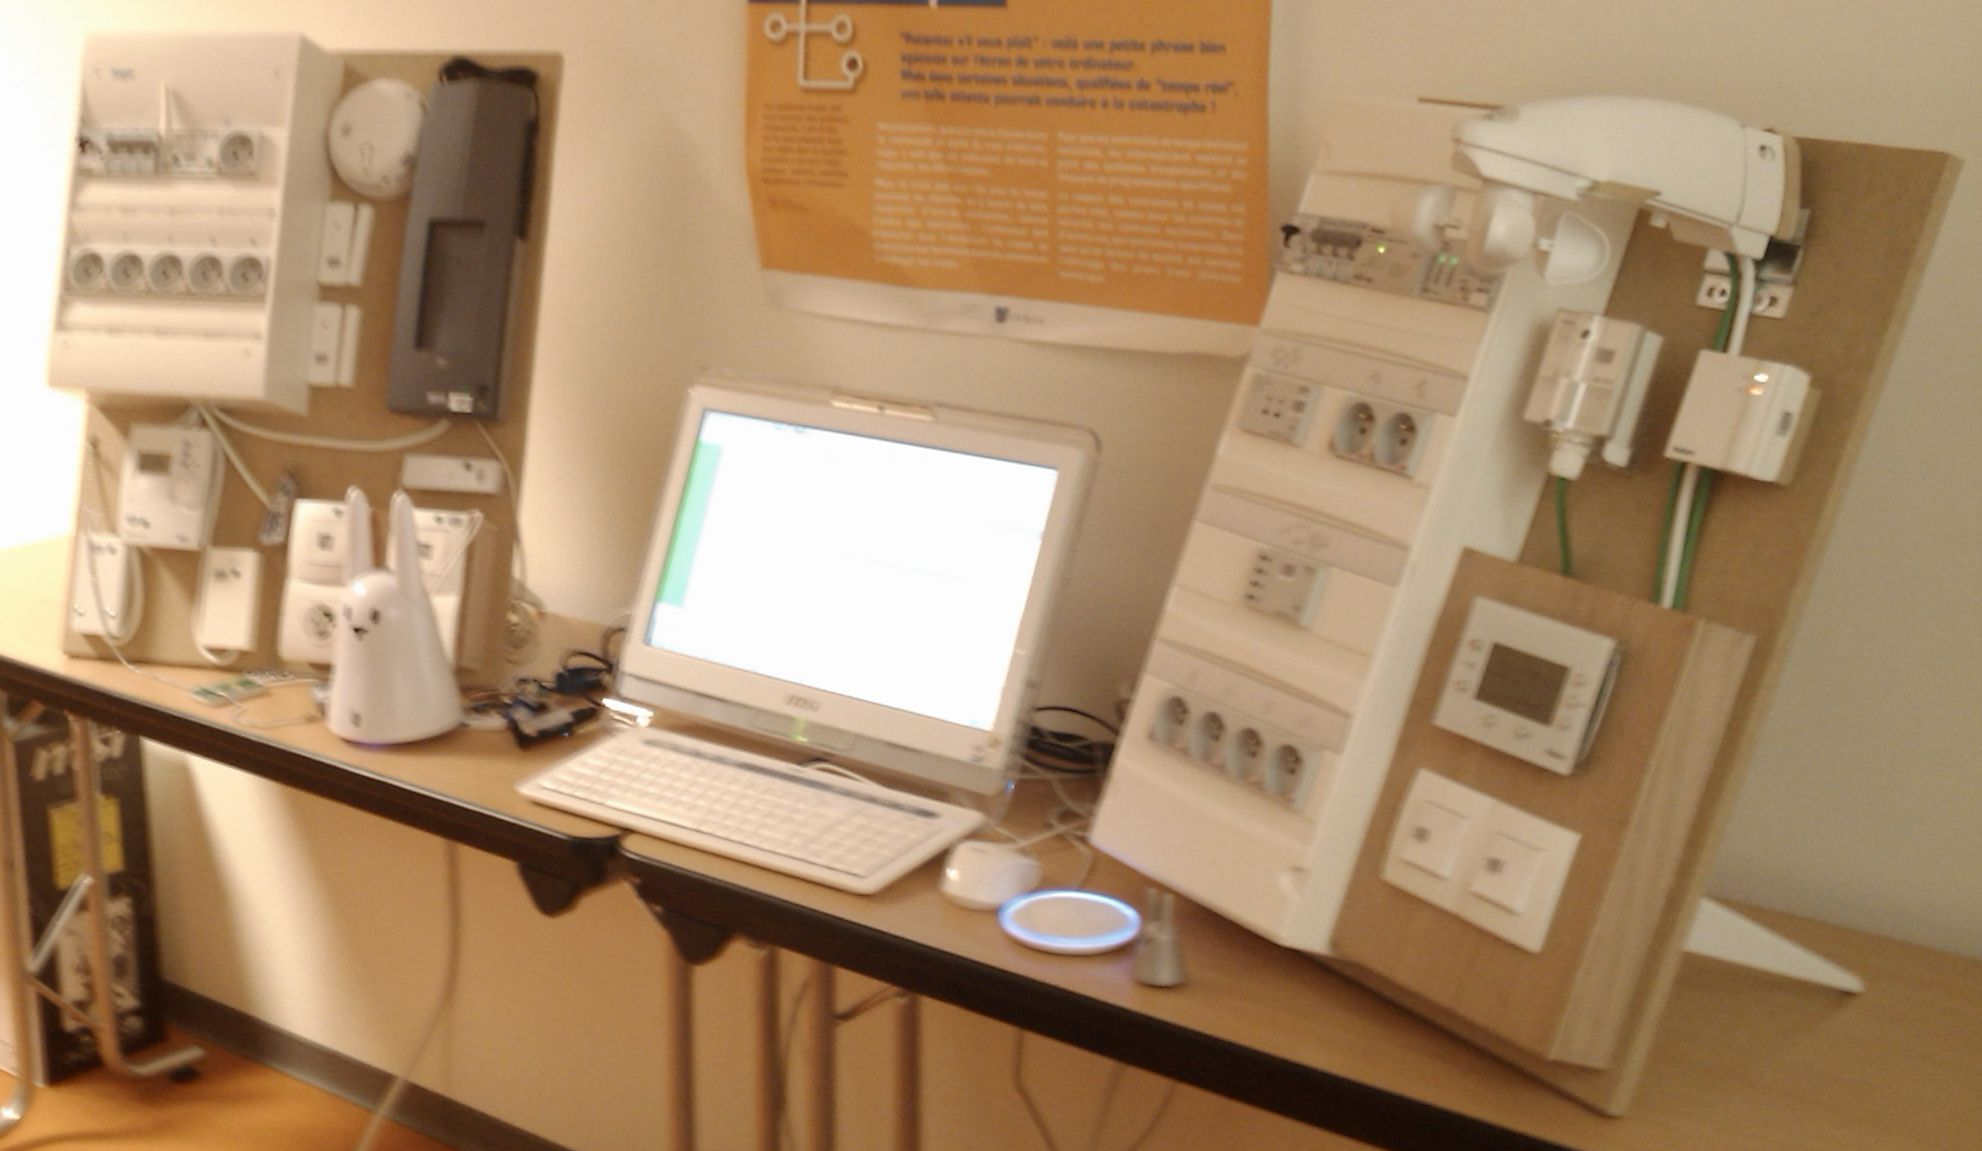
\includegraphics[width=\textwidth]{part4/pics/maquettes.jpg}
\caption{Equipments available for the study}
\label{fig:equimentsForTheStudy}
\end{figure}

\subsection{Delta Dore equipment}

The Delta Dore mock-up, visible on the left side of picture~\ref{fig:equimentsForTheStudy}, was set up with devices from heating, alarm, security and automatism functional domains. Here is the description of all the elements.\\
\begin{itemize}
\item A {\it DRIVER 210 CPL + TYDOM 520} heating controller, on the bottom left corner of the mock-up, controls two heater receivers: a {\it TC51089} \gls{plc} receiver, and a {\it RF660FP} radio receiver.
\item The big black box on the top right corner of the mock-up is a {\it TYXAL CSX40} alarm, which collects information from several sensors. A {\it DOFX} smoke sensor, and two {\it MiniCOX} door sensors, visible on the left side of the alarm. The last sensor is a {\it DFX} water leak sensor (green object on the table, under the mock-up).
\item One {\it TYXIA 442} light dimming transceiver, and a {\it TYXIA 411} timed power switch, both hidden behind the rabbit.
\item Not visible in the picture, two remote controls. One {\it TYXIA 110} with a single ON/OFF button, and a {\it TYXIA 141} with four.\\

\end{itemize}

All these elements use the X2D protocol, owned by of Delta Dore, to communicate on both PLC and radio media. Since the protocol is not public, Delta Dore lent us a research and development product, able to communicate in both ways (listen and act) on the X2D network.\\

\subsection{KNX equipment}

The second mock-up, on the right side of the picture, is made of KNX compatible products only, mainly from the manufacturer Theben and some from Siemens.\\

\begin{itemize}
\item On the top right corner of the KNX mock-up is an outdoor weather station. This weather station gives information about the wind, the rain, the temperature, and the light value. This information can be provided whether periodically or when a value changes slightly.
\item Just under the weather station, on the left, the {\it LUNA 113} is a light sensor for the outside. On its right, an {\it AMUN 7160} provides information about temperature, humidity and $CO_2$ rates inside the house.
\item Going down the right side comes the {\it VARIA 826 WH KNX}, which is an ambient controller. It allows for changes in the heating regulation values, reading information from the weather station and many other appliances.
\item The four switches, in the bottom right corner of the mock-up, are controlled by a {\it TA 4}.
\item The electric panel includes three other devices. An {\it RMG4s} device controls the four power sockets, at the very bottom of the panel, with a On/Off behavior only. Above this device, a {DMG 2} controls the dimming of the two sockets on its right.
\item Hardly visible on the top of the panel, a Siemens {\it EIB/IP N148/21} gateway makes it possible to access the KNX network through an IP connection. Helped by the Calimero~\footnote{http://calimero.sourceforge.net} framework, it enables a programmatic control on all the devices, and allows the user to listen for events on the KNX network.
\end{itemize}

\subsection{Other equipment}

The link between all of these devices is made by \enti{}, but it still requires an environment for its execution. Several other devices are available in this experimental setup.

\begin{itemize}
\item An all-in-one PC {\it MSI Wind Top}, with a touch screen, an Intel Atom 230@1.6GHz CPU, 1Gb RAM and Ubuntu 9.10 (Linux kernel: 2.6.31-17-generic) for the operating system. 
\item An {\it Icon 225} 3G USB modem, used only for sending short text messages
\item A Nabaztag:tag, the big rabbit in the picture, able to synthesize a voice from a text, and used to provide feedback to the user. A Nanoztag with a Mir:ror (little grey rabbit and round blue base) are used as an \gls{rfid} tag and an RFID reader respectively.
\item An Ethernet router to connect the KNX mock-up and the touch-screen.
\end{itemize}



\section{Interoperability issue}
\label{subsec:interop}

The first problem that the story of Mrs. P emphasises, is the connection of three heterogenous devices.

\subsection{Test Environment}
To evaluate \enti{} on this issue, we made use of the Tyxia 110 remote control from the Delta Dore mock-up, the 3G modem to send text messages and the Nabaztag:tag rabbit to provide feedback to the end user.\\
Nothing in \enti{} was already available to access these products.\\
The MSI Top touch-screen was used for the deployment of the test.

\subsection{Resolution Protocol}

{\bf Driver creation}\\
Each product used in this test is from a different manufacturer. Thus, three drivers had to be created, as described in section~\ref{subsec:useOfDrivers} of the contribution.\\

The driver enabling the use of the Tyxia 110 makes use of the gateway offered by the manufacturer, making it possible to listen on the X2D network. This gateway was delivered with a Java API, which simplified the creation of the driver. Indeed, the driver just consists of the creation of a listener and of a class to handle the implementation and the model of the remote control device. The Tyxia 110 component has a unique output port {\it pressed}, and can be customized to specify the parameters to be sent through the output port when the button is pressed.\\

The second element, the 3G modem was considered as a simple modem. The sequence of {\it AT} commands to be sent to the modem, to send a short text message, was collected from the modem documentation. With the help of a serial communication library in Java (RxTx), the component was implemented, and decorated with modeling annotations. The Icon 225 component representative offers a unique input port {\it send}. This port admits one parameter: the text of the message to send. The receiver's phone number is given as a parameter to the component.\\

The Nabaztag:tag rabbit is the last element in this test and is used to provide feedback to the final user. The web-service API of the Nabaztag rabbit provides a Text-To-Speech facility that can generate and return an MP3 file. Indeed, the rabbit is able to either, directly synthesize a voice from a text or generate a file containing the voice synthesis, for it to be played later by the rabbit. The component standing in for the rabbit thus proposes a {\it generate} input port. The action of this port is to call the text-to-speech facility with the text passed through the port as a parameter. The generated MP3 file is then returned through an output port called {\it generated}. A second input port, {\it play}, can be used to ask the rabbit to read a text or an MP3. If a text is given in parameter, the synthesis is made on the fly.\\

\begin{figure}[h!]
\centering
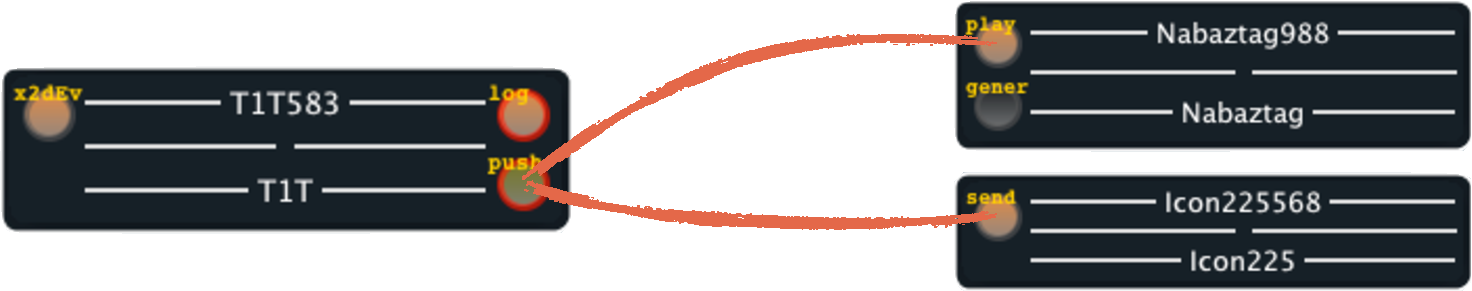
\includegraphics[width=.7\textwidth]{part4/pics/validInterop}
\caption{Components used in the interoperability experiment}
\end{figure}

{\bf Connection of the elements}\\

An instance of each element of the assembly is created in the model. The Tyxia 110 is customized to send two parameters through its output port on activation: the text "Your request has been sent to your daughter." for the rabbit, and "Your mother is requesting a call from you." for the Icon 225.\\
This message with the two parameters is forwarded to a dispatcher, which triggers in parallel the {\it send} input port of the Icon 225 instance, and the {\it play} input port of the Nabaztag. Each component collects the parameter it is interested in and carries out the required action.\\

\subsection{Results}

At first sight, the connection of a generic remote control, an electronic rabbit, and a short message modem is not that obvious. Industrial partners of the project were baffled by this requirement, because it implied that they develop an ad-hoc device. This is not viable when targeting a provision of specialized solutions for each person's needs.\\
%\enti{} makes this problem quite easy to solve.\\

In this example, three drivers had to be developed to be able to get components in the model. Each driver can now be augmented to provide more products from each manufacturer. The development of drivers, once done, is never to be done again. Components can also be reused in other contexts, because of their independence and the avoidance of direct connections. For future applications, this signifies a great gain in time.


\section{Evolution issue}
\label{subsec:evolution}

The evolution in this use case is due to a change in Mrs P.'s needs. She wants the lights to be automatically switched on when she presses the remote control. This requirement is related to a feeling of safety when lights are on at night.\\

\subsection{Test Environment}

This evaluation makes use of the previous devices involved in the interoperability evaluation.\\
In addition, the RMG4s of the KNX mock-up are integrated in the application.

\subsection{Resolution Protocol}


No KNX product had been used for the moment. So, the first task was to create the driver to control KNX equipment and obtain a model representative for the RMG4s (presented in figure~\ref{fig:rmg4s} a few pages back). Once the component is ready, it has to be deployed.\\
Thanks to the Model@Runtime layer, the technician responsible for the addition of the new functionality retrieves the current model of the running application, using a TCP/IP remote access. He then adds an instance of RMG4s and connects all {\it on} input ports to the dispatcher already present. In this configuration, all lights controlled by the RMG4s are lit when the Tyxia 110 button is pressed, in addition to the text being sent and the rabbit speaking.\\

\begin{figure}[h!]
\centering
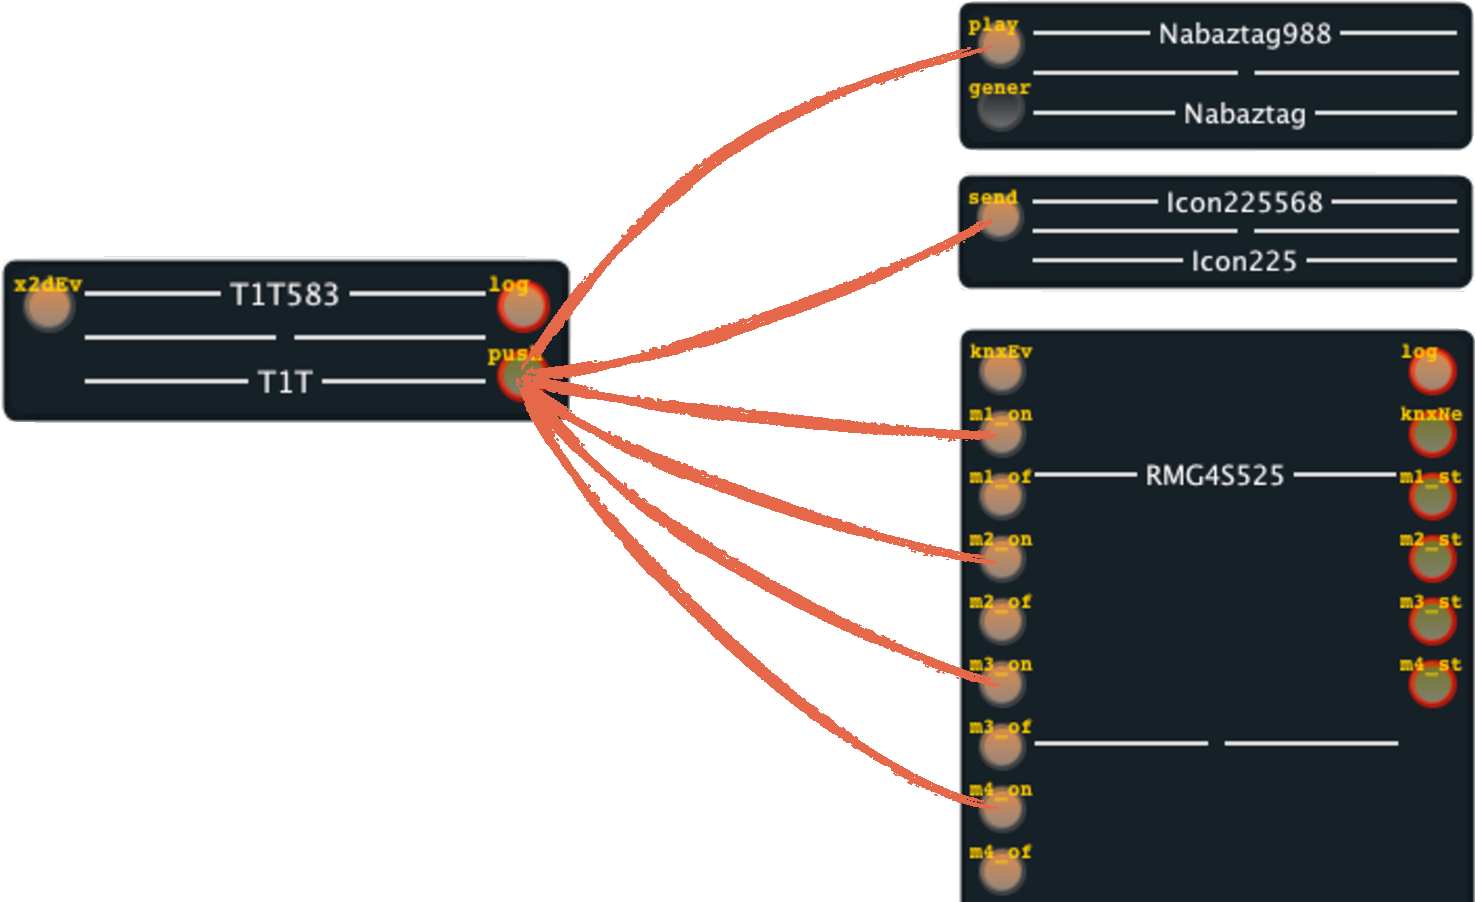
\includegraphics[width=\textwidth]{part4/pics/validEvol}
\caption{Components used in the evolution experiment}
\label{fig:validEvol}
\end{figure}

For the last step, the technician sends back the model to the runtime of \enti{} in the home. Once all checks are passed, the runtime downloads the newly-created component type and its driver, in order to create and connect the instance. All this procedure is transparent for Mrs P., who is called just before and after the operation to keep her informed. The OSGi runtime prevents any service interruption.

\subsection{Results}

Again, a driver had to be created as well as a component to handle the RMG4s. Thanks to the Model@Runtime engine, the technician was able to collect the model and modify it. He then asked the runtime for the deployment of the new model. Realized through a TCP/IP connection, this evolution could have been realized remotely. This ability reduces the disturbance for the helped person, and can reduce the time from the query to the realization.\\
For this experiment, the communication with the runtime used a TCP/IP connection, which may not be that easy in real life.


\section{Adaptation issue}
\label{subsec:adaptation}

The behavior of the lights was sub-optimal after the deployment of the evolution. Indeed, the lights were switched on, whatever the period of the day, every time the remote control was pushed. To remedy this issue, an adaptation mechanism (presented in \cite{Nain10a}) was deployed. This mechanism changes the configuration of the system, according to the external lighting value sensed by a KNX outdoor weather station.

\subsection{Test Environment}

In addition to the previous equipment, selected for interoperability experiments and evolution concerns, the outdoor KNX weather station is now included in the configuration.

\subsection{Resolution Protocol}

The driver for KNX products already exists. The unique thing to implement is a component representative for the weather station.\\

The Model@Runtime engine offers means to connect reasoners. A reasoner is able to modify (or ask for the modification of) the running system configuration. The decision is made locally according to some contextual information. This information can be as simple as a value change, or as complex as an aggregation of events.
For this evaluation, a reasoner has been created to modify the connections of the {\it RMG4S} according to the period of the day.\\

The system is currently composed of five components. A {\it TYXIA\_110} remote control, a dispatcher connected to a 3G USB stick to send texts, and to a Nabaztag rabbit to inform Mrs P. In addition, the RMG4S makes it possible to control the lights. {\bf At night}, this configuration is the one required. {\bf During the day}, the RMG4S should not be activated, and the connections with the dispatcher have to be removed.\\

\begin{figure}[h!]
\centering
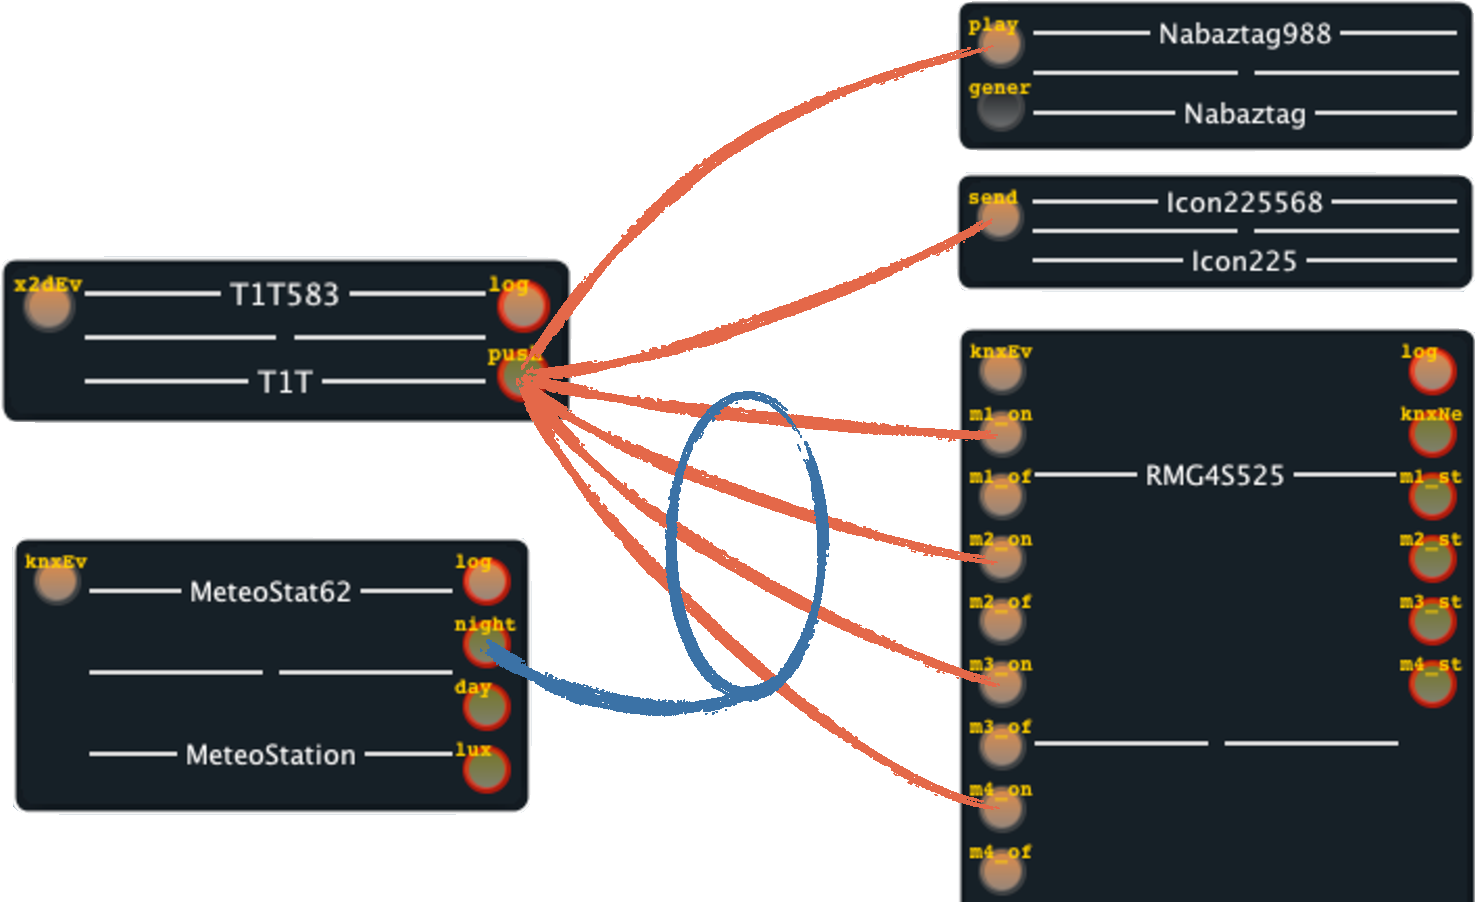
\includegraphics[width=\textwidth]{part4/pics/validAdapt}
\caption{Components used in the adaptation experiment}
\end{figure}


The weather station has been added to the system as described in section~\ref{subsec:evolution}.\\

To be able to perform execution time bench testing, the experiment including the reasoner was deployed from scratch.
The MSI Top was cleaned of any previous binary element and restarted. The deployment was then realized as follows:\\

{\bf Initial Deployment} The initial deployment is realized during the day. The model deploys only the remote control, the rabbit, the USB stick, the dispatcher, and the weather station. In this configuration, the elderly person can ask for help by pressing the Tyxia 110 button, just as before, but no light is switched on.\\
 
{\bf At night} The reasoner adapts the system to the new conditions. It changes the model by adding an RMG4S instance and all necessary connections to the dispatcher.\\
 
{\bf Day} When the day returns, the reasoner removes the connections and the instance of RMG4S.\\

\subsection{Results}

Figure~\ref{figure:bench} presents the execution times measured while a sequence of reconfigurations of the system was run. This sequence consisted of five steps. After the initial deployment (\textit{State 1}), the scenario iterates night states (\textit{State 2} and \textit{State 4}) and day states (\textit{State 3} and \textit{State 5}) during the next two days.\\

\begin{figure}[h!]
\centering
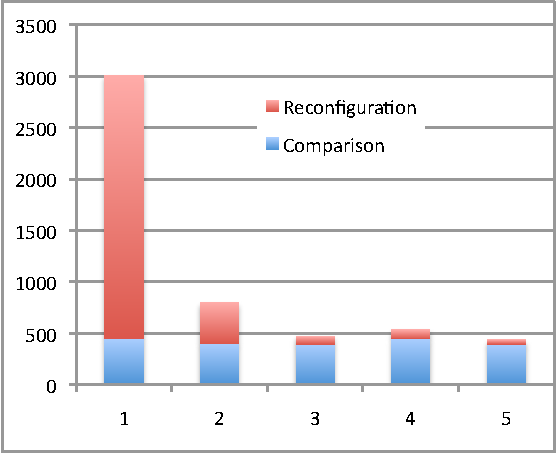
\includegraphics[width=7cm]{part2/pics/benchs_graphic3}
\caption{ Time (in ms) spent in Configuration Comparison and Actual Reconfiguration}
\label{figure:bench}

\end{figure}

As the  worst case scenario has been considered, the system is initially empty. Starting from scratch, all components need to be deployed during the initial configuration. In particular, all the component types have to be downloaded and checks have to be performed on the entire model. It explains the rather long reconfiguration time of step 1:  2.5 seconds. \\

The first reconfiguration (day $\rightarrow$ night, step 2) implied the deployment of an instance of RMG4S and the creation of bindings. As this component has never been used before, its component type is not present and has to be downloaded. All other components already deployed are reused. The downloading and deployment of the component type, plus the instance creation and its bindings to the dispatcher, are realized in less than 400 ms.\\

The next 3 reconfigurations (night $\rightarrow$ day $\rightarrow$ night) are much faster. Step 3 simply consists in unbinding and removing the RMG4S component. Step 4 is similar to step 2. Component types are not uninstalled. The RMG4S component type is thus immediately available for an instance creation. Step 5 is similar to step 4. The actual reconfiguration time of these steps is less than 100 ms.\\

For each reconfiguration, a model comparison is performed by the Model@Runtime engine, prior to the real deployment. This comparison detects changes and creates the commands' sequence for the transition. This model comparison takes an almost constant time of 400 ms. Executed before the actual reconfiguration, the comparison delays the reconfiguration of the system, but does not impact the duration of dynamic reconfiguration. \\



\section{Openness issue}
\label{subsec:opening}

As presented in section~\ref{sec:usecase}, the system was required to expose the devices on both \gls{upnp} and \gls{dpws} networks. The next two sections describe how components have been automatically wrapped to be available on these networks. They report an actualized version of the work presented in~\cite{Nain08a}.


\subsection{UPnP export}

UPnP~\cite{UPNP} is based on a discovery-search mechanism. As a UPnP-Device joins the UPnP network, it sends an XML description file to all UPnP-ControlPoints. This file presents the device with information such as manufacturer, device type, device model, or its UUID. Most of times a UPnP-Device is self-contained.\\
It is able to describe itself and the services it publishes on the network. The description structure, visible on the upper part of figure~\ref{fig:upnp-mapping}, is organized as follows.\\
UPnP specifications allow devices to contain other devices (called embedded devices). In this case, the container (called the {\it rootDevice}) takes the responsibility for publishing information about itself and each device it embeds.\\
Each service a device can offer has to be described in a separated file. This file characterizes all the UPnP-Actions the service renders, and all the UPnP-State Variables used by these actions. UPnP-Actions can admit parameters. These parameters have a direction (in or out), a name, and a related StateVar. UPnP-StateVars handle information such as value types, or lists of allowed values for a parameter.\\


\subsubsection{Test Environment}

This experiment required some devices to be deployed on the runtime for them to be exported. We chose to fix the system in the night state of the previous experiment, thus with a maximum of devices present in the system.\\
This test also required a third party tool to act as a UPnP external control point. This was the touch screen provided by Mrs P.'s son. Since \enti{} was deployed on the MSI Top, we made use of a toolkit from Intel: "Intel® Tools for UPnP Technologies (Build 2777)". This toolkit is no longer maintained and is only available for Windows.

\subsubsection{Resolution Protocol}

{\bf Mapping UPnP devices to \enti{} devices}\\
Although \enti{} devices and UPnP devices are quite similar, they are not exactly aligned in their structures. However, the mapping (blue arrows in figure~\ref{fig:upnp-mapping}) was quite natural. \enti{} devices were mapped on UPnP devices.\\
\enti{} devices can provide two kinds of ports: service and messages ports. {\it NB: only input ports are considered here}. Services ports are composed of operations. This kind of ports was associated with its UPnP equivalent, namely Service for the port, and Action for the operations. The closest UPnP element to handle message ports from \enti{} is the concept of {\it Actions}. Indeed, a message port provides only one service/action. As a consequence, there are as many services as there are message ports created. Each service proposes a single action, which connects to the message port.\\

\begin{figure}
\centering
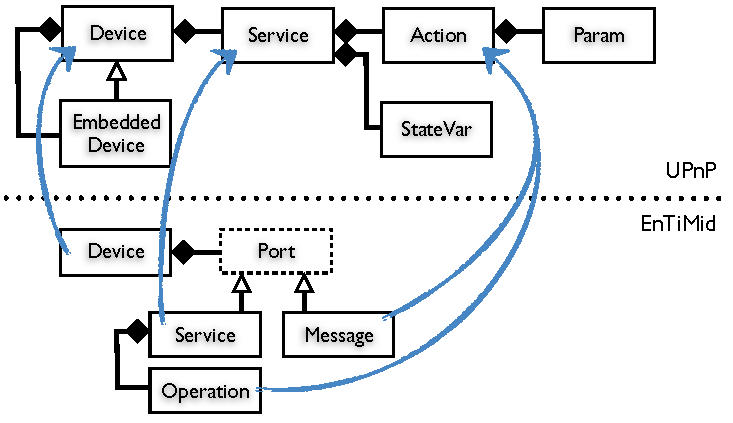
\includegraphics[]{part4/pics/UPnPMapping}
\caption{Mapping UPnP-EnTiMid}
\label{fig:upnp-mapping}
\end{figure}

{\bf Generation of description files}\\
In \enti{}, each component is described by a model. The model is a graph of objects at runtime and is serialized in an XML file. The generation of the XML description file for UPnP is thus quite natural.\\
The service descriptions are the first files to be generated. For each \enti{} service, a new file is created. Operations of the service are then described in the UPnP formalism. Not all operations are described, due to a sometimes complex translation between \enti{} and UPnP runtimes. In any case, all simple methods are included in the description. In the same way, a new service file is created for each message port. The service takes the name of "<port>on<component>" for the services to be differentiated. Each service of this kind is composed of a unique action whose name is identical to the one of the port.\\
Afterwards, a separate description file is created for each component available on the system. The description of a device in UPnP is threefold. The first part provides general information about the product such as the name of the manufacturer, a brief description, the model type, the model number, or its serial id. If not available in the model, these elements are automatically generated, or completed with default values. The second part contains the list of the services a device provides. This description makes reference to the service description files previously generated. The last part contains information about the embedded devices. For each of them, the two previous parts have to be specified.\\

When a UPnP-ControlPoint starts, it broadcasts a query for descriptions of devices available on the network. The UPnP wrapper then sends the description files of all devices and services provided in response.\\

{\bf Runtime elements}\\
The generation of description files is necessary, but not sufficient for UPnP queries to be forwarded to the real device. Indeed, no connection was made between the real runtime component standing for the devices and the UPnP network. To cope with this issue, virtual abstract \enti{} components are created at runtime. Each real device exported on the UPnP network is linked to an abstract component responsible for the handling of communications between the real device and the network requests. These abstract components only have output ports. {\it i.e.}: an output port is specially created on the abstract device to be connected to each input port of the real device exported on the UPnP network.\\
Then, queries are routed by the UPnP exporter to the abstract component in charge of the concerned device. The abstract component activates the input port of the real device according to the request.\\

\subsubsection{Results}

Once the wrapper is deployed on the MSI Top, the Nabaztag rabbit, the 3G USB stick and the RMG4S were all made available through the UPnP network. Indeed, we were able to view and act on these devices from a remote PC equipped with Windows, and the Intel UPnP toolkit.\\
The low number of tools that accept the discovery of self-describing UPnP devices can be a limitation for the use of this wrapper.


\subsection{DPWS export}


\gls{dpws}~\cite{DPWS} defines a minimal set of implementation constraints, to enable secure Web Service messaging, discovery, description and eventing on resource-constrained devices. Its objectives are similar to those of \gls{upnp}. The difference is that DPWS is fully aligned with Web Services technology and is designed to work upon a web-service transportation protocol. It also includes numerous extension points, to allow for seamless integration of device-provided services in enterprise-wide application scenarios.\\
From a conceptual point of view, the DPWS structure is close to that of UPnP, described in figure~\ref{fig:upnp-mapping}. Consequently, the mechanisms to map \enti{} devices and their \gls{dpws} representative follow the same idea. Nevertheless, the generation process is different. Publications to the DPWS network have been realized thanks to the WS4D project~\cite{ws4d}. In their approach, each DPWS-compatible device has to extend an abstract DPWS device, proposed by the framework they provide. The reason is that this abstract component handles all web service-specific communication concerns. The creation of a virtual component is not sufficient in this case. A source code has to be generated.\\

\subsubsection{Test Environment}

Since UPnP and DPWS are very close in terms of needs for devices to be exported, the same set of devices was selected for this experiment.\\
As for UPnP, we made use of an external tool to check that the export of devices was made properly. The experiment was carried out using a second PC equipped with a DPWS explorer\footnote{http://ws4d.e-technik.uni-rostock.de/dpws-explorer/} to list and act on published devices.

\subsubsection{Resolution Protocol}

{\bf DPWS devices creation}\\
For each device, service and operation, a Java class has to be generated. According to the element they represent, classes must extend {\it HostedService} for services, {\it HostingService} for devices and {\it Action} for operations. Parameters are instances of the class \textsf{Parameter}. Luckily, all these classes still can be generated with an automated process. To achieve the code creation, the JET Framework has been used. Templates of DPWS files were set up and they are used at runtime to produce Java classes.\\
More than just Java classes, the generated files are also implementations of new component types. These types are the wrappers of real devices for DPWS. These components are thus responsible for the direct connection between model elements and DPWS controllers.

{\bf Compilation and use}\\
The generation process produces Java classes, but no binary code. These classes still have to be compiled to be useful at runtime. The decision was made to embed the JDT compiler provided by Eclipse. As a result, the bundle to export devices through DPWS is a bit heavy. The compilation is also resource-consuming for quite a small computer device. Once compiled, these classes are packaged into a bundle, which is then deployed on the OSGi runtime.\\
Classes are then handled just as classical components. The tool asks for new components to be added in the runtime, and they are bound to the device  they export.\\

\subsubsection{Results}

Obviously, this is not optimal but it works, since we were able to see all devices and act on them using the DPWS Explorer tool. Other solutions involving more powerful servers in charge of the transformation from a model representation to a component type bundle have been proposed, but not yet completely realized. In any case, the principle is just to extract a tool chain that already works.\\


\section{Threats to validity}
\label{sec:theatsToValidity}

\subsection{Internal threats}

\subsubsection{Variability management}

Variability management, described as being an important issue in home automation for assisted living is not addressed in this experiment.
Indeed, the scenario considers a unique deployment, for a single person, in a single home. A second round of definitions of a more global scenario may have stressed this requirement for variability management.\\
Nevertheless, a lot of work has been carried out to try to cope with this issue, such as an approach using Aspect-Oriented Modeling presented in \cite{Morin09a}. Other perspectives to address this question are presented in section~\ref{sec:archiSynth}.

\subsubsection{Scalability}

The scenario did not highlight any issues about the distribution or scalability of the solution for deployment on a town-wide or even a countrywide scale. 
This scalability validation will be addressed in the future with real deployments.\\
The MSI Wind Top, on which the experiments have been led, may not be the unique platform on which to test \enti{} and a large-scale vision scenario would have highlighted this.\\

\subsubsection{Safety and Security}

Voluntarily, we decided to distance ourselves from access security and privacy considerations. Not because they are not essential, but because they impose such heavy constraints that the search for a technical solution may have been compromised. Now that the system is clearly designed and that the proof of concept has been validated, work to secure communications and data has to be realized prior to any real deployment.\\

Concerning safety, our experimentations did not require complex checks on models. Only simple structural checks, to find cycles for instance, were implemented and used.
In our approach, type checkers and validation policies have been designed to be customized according to the application domain and its constraints. Thus, their complete definition would have been useless in the context of the experiment. In the case of real deployments, they have to be completed to verify that no configuration identified as a case of failure is asked for deployment.

\subsection{External threats}

\subsubsection{Validity of the scenario, real deployment}

The experimentation scenario, even when defined in collaboration with several players in the AAL domain may not consider all cases. The interface between people coming from a technical field and people coming from social field is quite difficult to find. Because people in social activities are not aware of what it is possible to do with technologies and because industrialists are not aware of the everyday problems the dependency of persons can raise, the discussions can rapidly come to a dead end.\\
The scenario validated for this study was accepted by all sides, but may be limited by the comprehension each side had of the problem.\\

\enti{} has been instantiated and validated on a virtual case. A real deployment would have highlighted other issues, other constraints not addressed in this evaluation. This real deployment is part of the perspectives for this work.


\subsubsection{Communications with smart devices}

Gateways are essential for us to be able to communicate with smart devices. For instance, the bi-directional communication with Delta Dore devices was made possible by an R\&D product. Otherwise, the {\it TYDOM 350}, an embedded web server, is the only device they commercialize to act on their devices. This one only enables users to act on devices through a web page interface. This product does not detect any event on the X2D network; it just acts on devices (with no acknowledgement by the way).\\
\enti{} is not able to use any device without a means of communication with it.

 

\section{Conclusion}
\label{sec:concluAAL}

An experimentation using real devices was set up by a collaborative work of the project's partners to evaluate \enti{} on a scenario as realistic as possible. Made with the background of each partner, this scenario was designed to stress several issues identified on this kind of integration systems.\\
\enti{} passed the main requirements highlighted by the scenario and required for such systems to be deployed. This validation comfort the idea of making \enti{} an integration platforms to offer customized solutions for each person's needs.\\
Some limitations due to the lack of real and large scale deployment have been identified. These limitations will probably be addressed by the project of the company in charge of promoting this technology in the industry.



\section{Implementation Metrics}

This section provides some lines of code metrics of Kevoree and EnTiMidd. These metics have been measured on Kevoree 1.5.0-SNAPSHOT and EnTiMid 3.0.0-SNAPSHOT on the 23rd November 2011.\\

\begin{tabular}{l||c|c|c|c|c}
Project & Scala & Java & Total & Part & Value \\
\hline \hline
Kevoree-Core & 8143 & 344 & 8487 & 11,54\% & 979,3 \\
Kevoree-Tools & 8483 & 6255 & 14738 & 22,22\% & 3274,65 \\
Kevoree-Extra(ecore) & 1275 & 126 & 1401 & 50\% & 700,5 \\
\hline \hline
EnTiMid-Core & 0 & 445 & 445 & 85\% & 378,25 \\
EnTiMid-Tools & 82 & 315 & 3197 & 75\% & 2397,75 \\
EnTiMid-Library & 0 & 2065 & 2065 & 80\% & 1652 \\
EnTiMid-Extra & 0 & 1091 & 1091 & 85\% & 927,35 \\
\end{tabular}\\
\\

As previously said, Kevoree can be seen as a generalization of EnTiMid. During the extraction, a deep refactoring have been realized to allow for future extensions.\\
EnTiMid has been specialized to address the domain of home automation. Thus, the most important par of development were paid in creating component libraries and extra APIs wrapping. For demonstration purposes, several additional tools had also been realized.

